\documentclass[12pt]{article}

\usepackage[margin=1.0in]{geometry}
\usepackage[parfill]{parskip}
\usepackage{amsmath}
\usepackage{graphicx}
\usepackage[font=bf]{caption}
\usepackage{changepage}
\usepackage{xcolor}



\begin{document}

\setlength{\parskip}{12pt}      % set paragraph skipping to one whole line



\title{A Kalman Filter for RSSI Tracking}
\author{Robert S. Huston}
\date{\today}

\maketitle

\vspace{24pt}

\begin{abstract}
This article investigates the application of a Kalman filter for estimating RSSI signal
levels acquired via a mobile device.
\end{abstract}



%-------------------------------------------------------------------------------
%
% Introduction
%
%-------------------------------------------------------------------------------

\section{Introduction}

The purpose of this article is to investigate the feasibility of applying a Kalman filter
to smooth a series of acquired RSSI readings of a nearby Bluetooth device. The RSSI readings
are captured using an iPhone running a simple iOS application that monitors Bluetooth signals
in its environment.

We use a Gauss-Markov process to model the RSSI acquisition behavior of a Bluetooth Low
Energy (BLE) device signal as seen by the mobile device. We use this model because its
autocorrelation function seems to match what we have observed from the signal behavior of
experimental RSSI data captured over time.

We then present two experiments that illustrate our findings.



%-------------------------------------------------------------------------------
%
% Gauss-Markov Process
%
%-------------------------------------------------------------------------------

\section{The Gauss-Markov Process}

A stationary Gaussian process that has an exponential autocorrelation function is called
a \emph{Gauss-Markov} process. If we designate $x(t)$ as a Gauss-Markov process, its
autocorrelation function is of the form

\begin{equation}
    R_x(\tau) = \sigma^2 e^{-\beta \, \lvert \tau \rvert}
    \label{eq:GM-autocorrelation}
\end{equation}

where $\sigma$ is the process mean-square value, and $\frac{1}{\beta}$ is the process time
constant. The Gauss-Markov process is a popular model because it fits a large number of
physical processes, and because it is has a simple mathematical description. It basically
describes a process where its values are more correlated when the time spacing between
successive measurements is small, and less correlated when the time spacing between
successive measurements is large.

The Gauss-Markov process has a spectral density function of the form

\begin{equation}
    S_x(s) = \frac{2 \sigma^2 \beta}{-s^2 + \beta^2}
    \label{eq:GM-spectral-function}
\end{equation}

From linear system theory, we know that if we can factorize a spectral density function
into LHP and RHP forms of the same factor function $G(\cdot)$:

\begin{equation}
    S_x(s) = G(s) G(-s)
    \label{eq:Spectral-factorization}
\end{equation}

then $G(s)$ is the shaping filter that shapes unity white noise into the spectral density
$S_x(s)$. Thus, for the Gauss-Markov spectral density, we have

\begin{equation}
    S_x(s) = \left ( \frac{\sqrt{2 \sigma^2 \beta}}{s + \beta} \right ) \left ( \frac{\sqrt{2 \sigma^2 \beta}}{-s + \beta} \right )
    \label{eq:GM-spectral-factorization}
\end{equation}

and so the shaping filter is

\begin{equation}
    G(s) = \frac{\sqrt{2 \sigma^2 \beta}}{s + \beta}
    \label{eq:GM-shaping-filter}
\end{equation}

and the corresponding differential equation is

\begin{equation}
    \dot{x} = - \beta x + \sqrt{2 \sigma^2 \beta} \; w(t)
    \label{eq:GM-differential-equation}
\end{equation}

where $w(t)$ is a unity white noise process.

The complementary solution is

\begin{equation}
    x_c(t) = e^{-\beta t}
    \label{eq:GM-complementary-solution}
\end{equation}

Hence, the discrete-time state transition function is

\begin{equation}
    \phi_k = e^{-\beta \tau_k}
    \label{eq:GM-state-transition}
\end{equation}

and the discrete-time process variance is

\begin{equation}
    \setlength{\jot}{10pt}
    \begin{aligned}
    Q_k &= E[w_k^2] \\
        &= \int_0^{\tau_k} \left ( \sqrt{2 \sigma^2 \beta} \; e^{-v} \right ) ^ 2 dv \\
        &= \sigma^2 \beta \left ( 1 - e^{-2 \tau_k} \right )
    \end{aligned}
    \label{eq:GM-process-variance}
\end{equation}



%-------------------------------------------------------------------------------
%
% RSSI Kalman Filter
%
%-------------------------------------------------------------------------------

\section{An RSSI Kalman Filter}

The Kalman filter implementation of a Gauss-Markov process model can be implemented
very efficiently since it involves only scalar arithmetic.

For the $k$th time point, we obtain a measurement $z_k$ at time $t_k$. We model our
measurement error with a variance $R_k$. At each time point, the filter provides a best
estimate, $\hat{x}_k$ and maintains a state estimate variance, $P_k$. We initialize the
filter with $\hat{x}_0 = z_0$ and $P_0 = P0$, where $P0$ is a suitably chosen value based
on empirical analysis.

Because our measurement is direct, the measurement transformation $H_k = 1$, and as such,
it will not be denoted in our filter equations.

For each acquisition event, $k$, we perform the following steps

1. Compute $\tau_k$:

\begin{equation}
    \tau_k = t_k - t_{k-1}
    \label{eq:KF-tau}
\end{equation}

2. Compute $\phi_k$ and $Q_k$:

\begin{equation}
   \phi_k = e^{-\beta \tau_k}
   \label{eq:KF-phi}
\end{equation}

\begin{equation}
  Q_k = \sigma^2 \beta \left ( 1 - e^{-2 \tau_k} \right )
  \label{eq:KF-Q}
\end{equation}

3. Compute predicted state estimate:

\begin{equation}
    \hat{x}_k^- = \phi_k \, \hat{x}_{k-1}
    \label{eq:KF-x-prediction}
\end{equation}

4. Compute predicted state estimate variance:

\begin{equation}
    P_k^- = \phi_k \, P_{k-1} \, \phi_k + Q_k
    \label{eq:KF-P-prediction}
\end{equation}

5. Compute Kalman gain:

\begin{equation}
    K_k = \frac{P_k^-}{P_k^- + R_k}
    \label{eq:KF-gain}
\end{equation}

6. Compute updated state estimate:

\begin{equation}
    \hat{x}_k^+ = \hat{x}_k^- + K_k \,(z_k - \hat{x}_k^-)
    \label{eq:KF-x-update}
\end{equation}

7. Compute updated state estimate variance:

\begin{equation}
    P_k^+ = (1 - K_k) \, P_k^-
    \label{eq:KF-P-update}
\end{equation}



%-------------------------------------------------------------------------------
%
% Experiments
%
%-------------------------------------------------------------------------------

\section{Experiments}

A simple iOS application was developed that enables an iPhone to continuously scan for
nearby Bluetooth devices, reading among other properties, their RSSI, UUID, and device
name properties. Each reading gets timestamped and logged to a file that an be copied to
a computer for further processing. A simple Python script was written to allow for the
selective processing and plotting of data based on device UUID.

Two experiments were then performed. The first experiment involved walking the scanning
iPhone (an iPhone Xs Max) away throughout the house (hallway and then dining room) from
the development MacBook Pro computer (kitchen) and then moved back again. The second
experiment involved taking both the scanning iPhone and a second iPhone outside and then
walking the scanning iPhone from the corner of the back yard to the second iPhone and then
away again. Figure \ref{fig:experiment-diagram} depicts a simple diagram of the walking
routes taken (shown in red) for each experiment. The distance values are approximate.

\begin{figure}[ht]
    \centering
    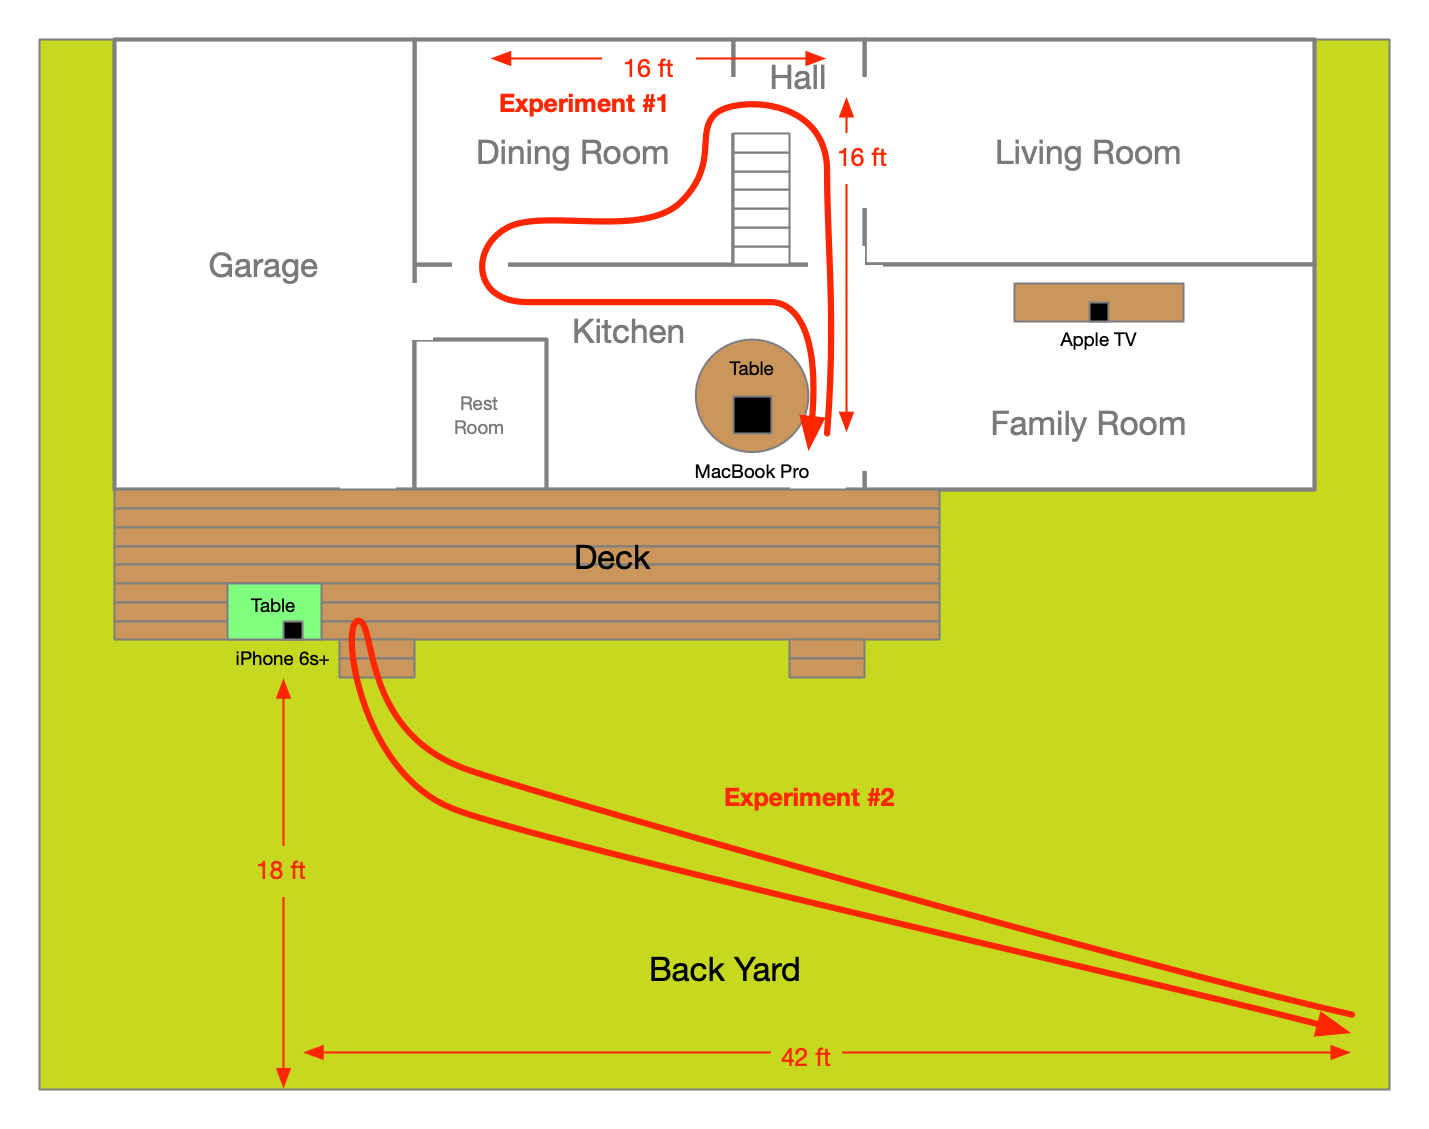
\includegraphics[width=1.0\textwidth]{RSSI-Experiment-Routes.png}
    \caption{Diagram of Experiment Walk Routes (Shown in Red)}
    \label{fig:experiment-diagram}
\end{figure}

In all cases, the RSSI Kalman filters were initialized with the following parameters:

\begin{center}
    \begin{tabular}{cccc}
        $P_0 = 5$ 
        &
        $\sigma = 10$
        &
        $\beta = 0.001$
        &
        $R = 10$
    \end{tabular}
\end{center}

One particular note about the second experiment was that the second iPhone screen was
active when the device was placed on a table on the deck before initiating the experiment,
but, by the time the walk from the corner of the yard had reached the second iPhone, it was
observed that the screen of the second iPhone had just gone to sleep. This can be seen in
the rate of the acquired data, where the "awake" condition produced more Bluetooth scan
responses than the "sleep" condition. This was a fortunate event, because it provided a
perfect data set to illustrate why a Gauss-Markov process model is suitable.

For the first experiment, the UUID of the development MacBook Pro (Red Green) was
monitored. The scanning iPhone was walked away from and then back to the computer. The
results can be seen in Figure \ref{fig:experiment-1-mbp}. The RSSI measurements are blue,
and the filtered RSSI values are in red.

\begin{figure}[ht]
    \centering
    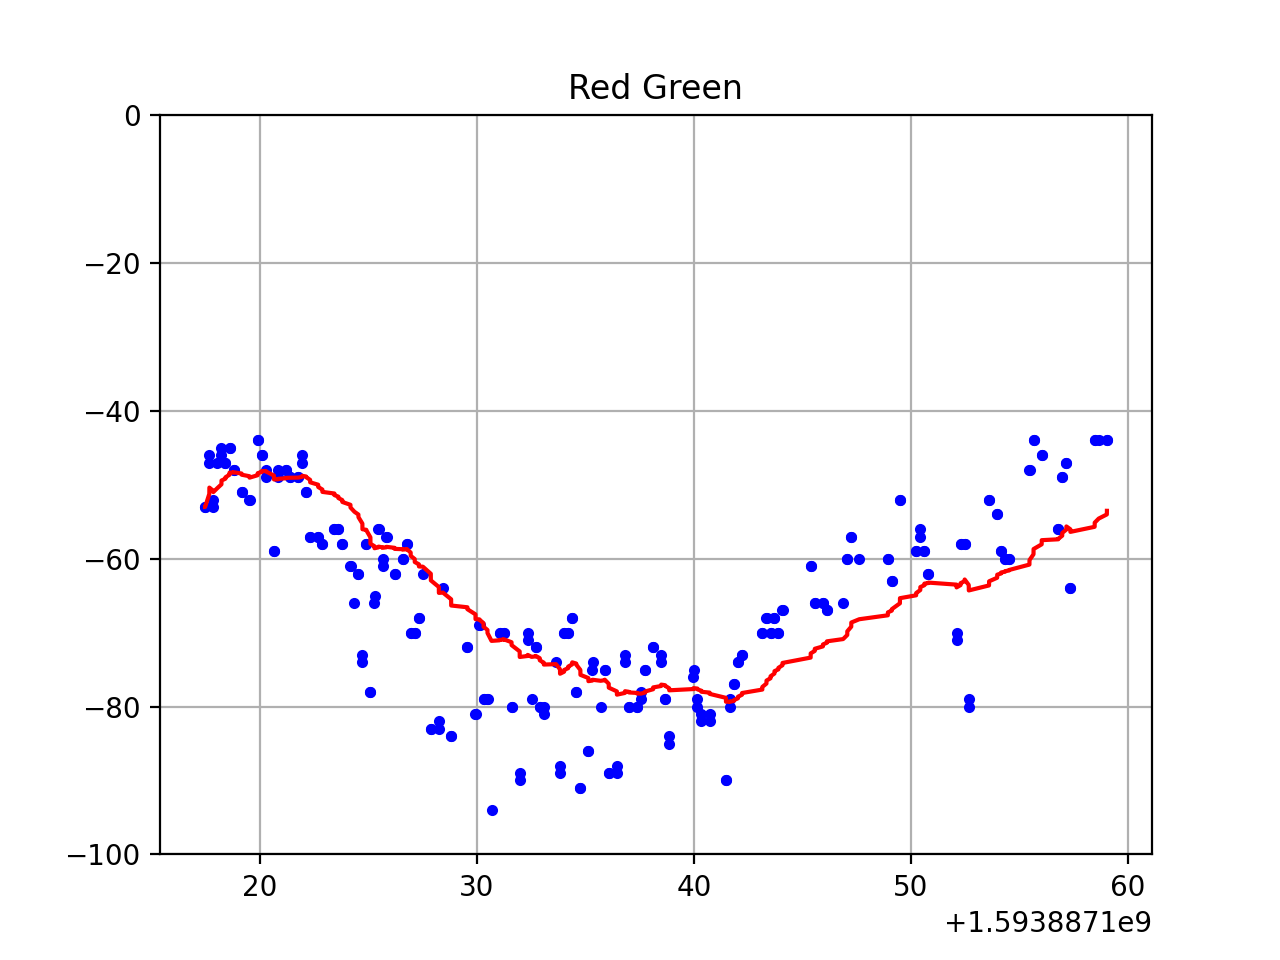
\includegraphics[width=1.0\textwidth]{Experiment-1-MBP.png}
    \caption{First Experiment - Scanning MacBook Pro from Indoors}
    \label{fig:experiment-1-mbp}
\end{figure}

For the second experiment, both the scanning iPhone and the second stationary iPhone
(an iPhone 6s+) were outside in the back yard. The scanning iPhone was walked from the
corner of the yard to the stationary iPhone and back again. As was stated previously,
the stationary iPhone screen went to sleep when the scanning iPhone reached the stationary
iPhone location. The scanning iPhone was then walked away back to the corner of the yard.
The results for the second iPhone can be seen in Figure \ref{fig:experiment-2-iphone}.

\begin{figure}[ht]
    \centering
    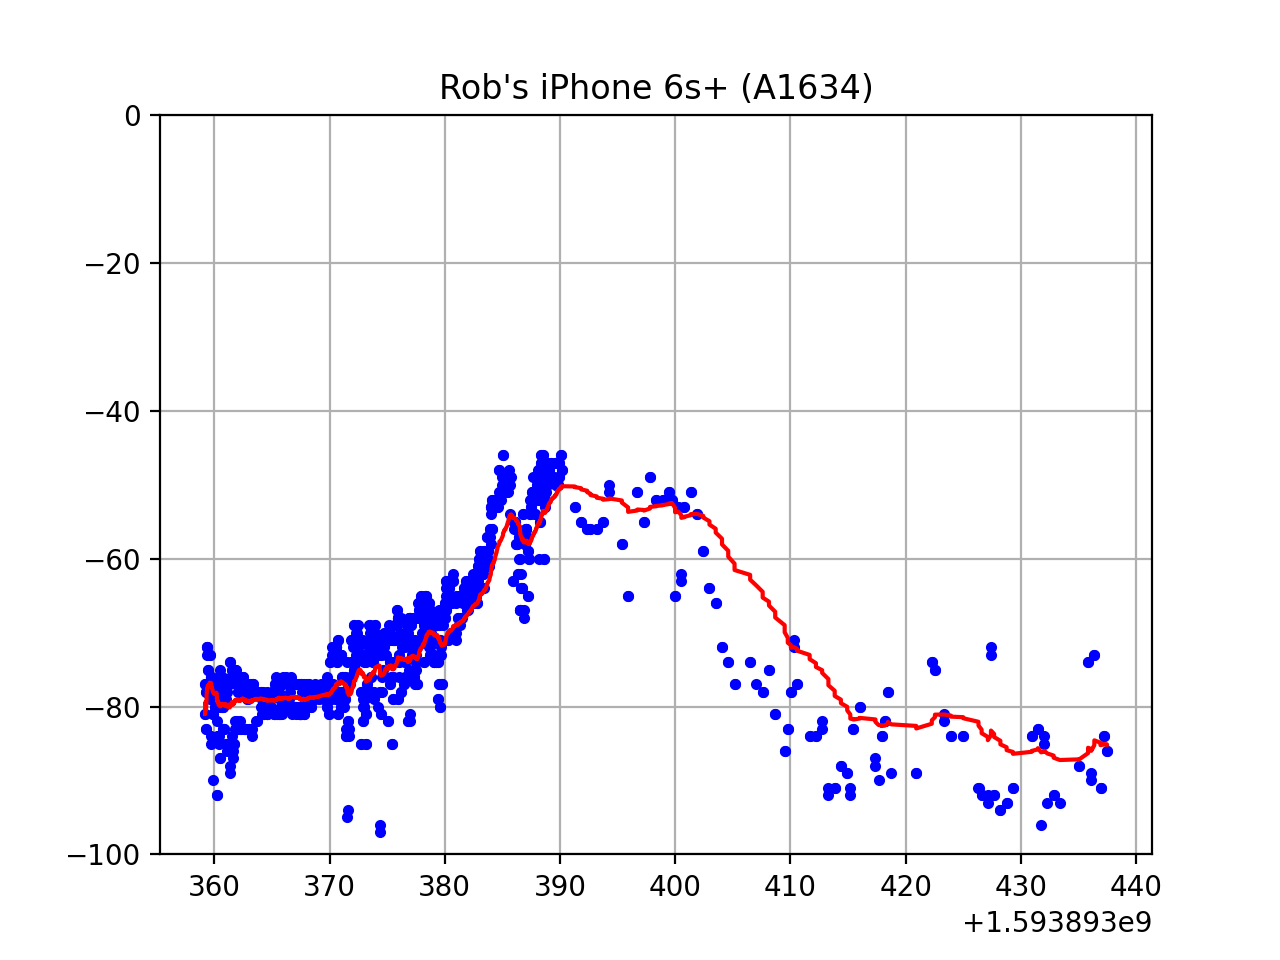
\includegraphics[width=1.0\textwidth]{Experiment-2-iPhone.png}
    \caption{Second Experiment - Scanning Second iPhone from Back Yard}
    \label{fig:experiment-2-iphone}
\end{figure}

Also available from the second experiment was the scanned Bluetooth signal data from both
the development MacBook Pro computer in the kitchen, and an Apple TV in the family room.
As shown in Figure \ref{fig:experiment-diagram}, both devices are in rooms that face the
back yard, and their distances from the scanning iPhone are comparable. The results for
the MacBook Pro can be seen in Figure \ref{fig:experiment-2-mbp}, and the results for the
Apple TV can be seen in Figure \ref{fig:experiment-2-atv}.

\begin{figure}[ht]
    \centering
    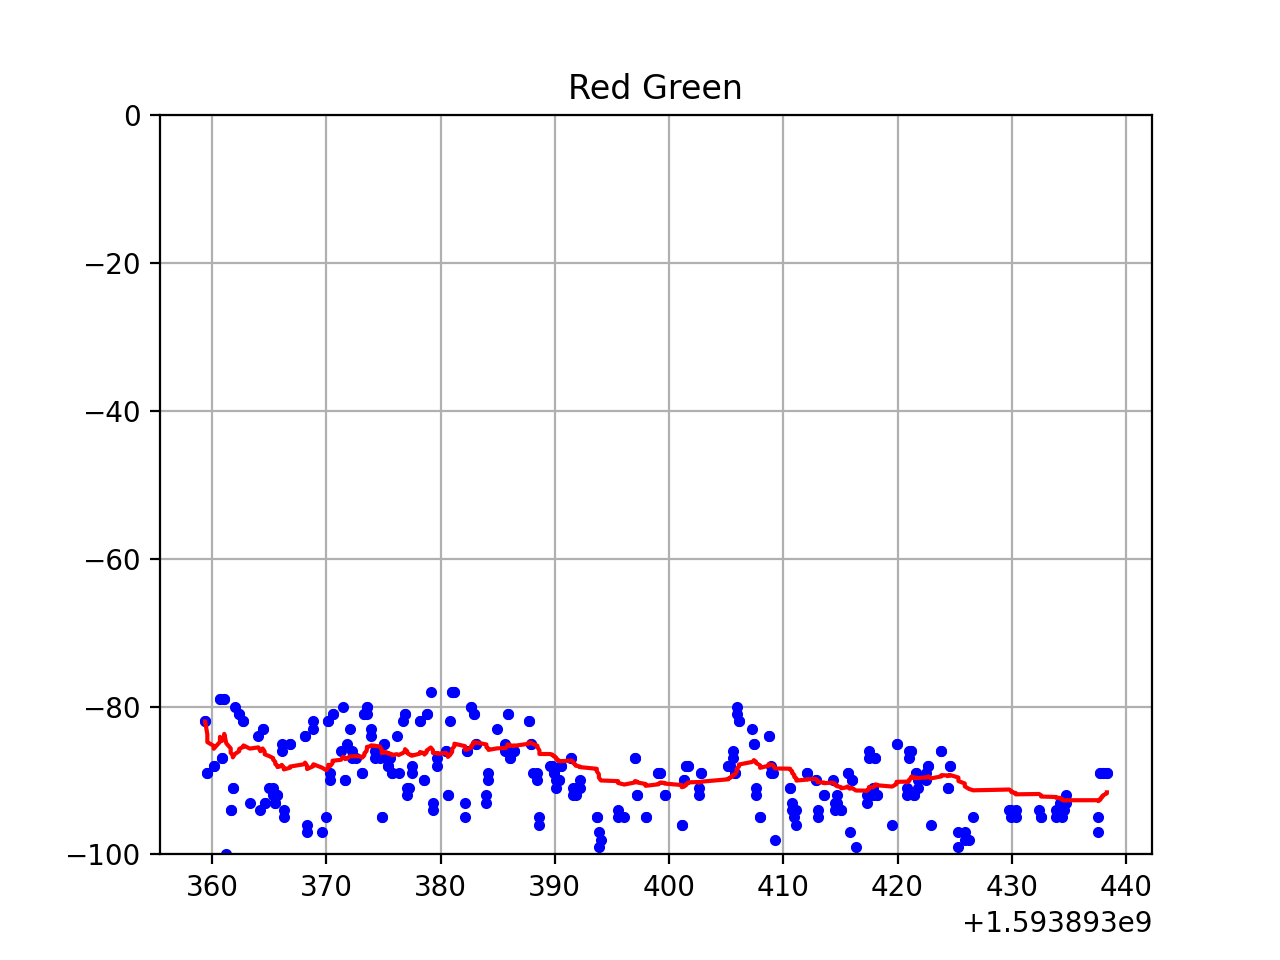
\includegraphics[width=1.0\textwidth]{Experiment-2-MBP.png}
    \caption{Second Experiment - Scanning MacBook Pro from Back Yard}
    \label{fig:experiment-2-mbp}
\end{figure}


\begin{figure}[ht]
    \centering
    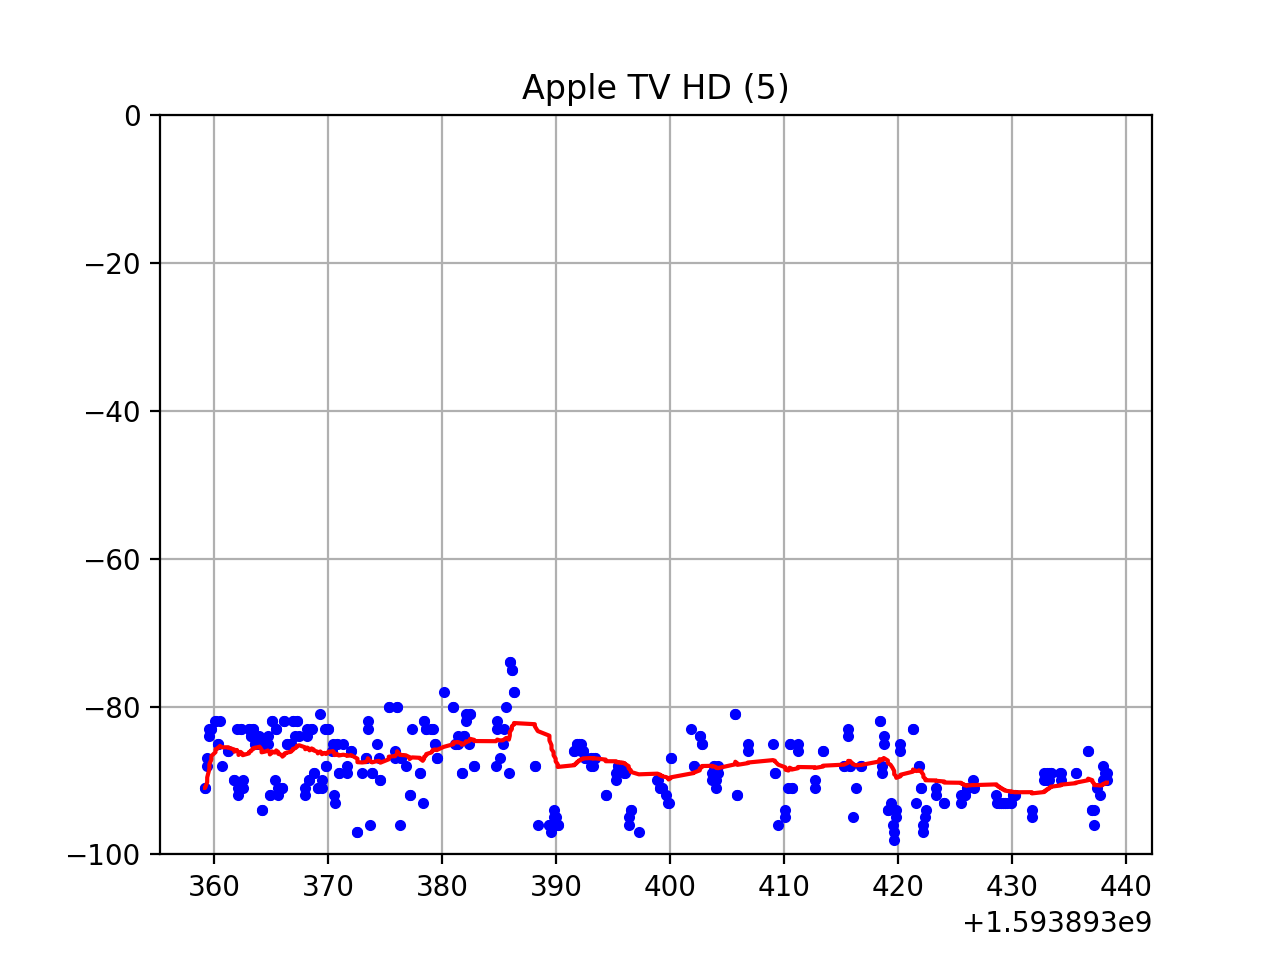
\includegraphics[width=1.0\textwidth]{Experiment-2-ATV.png}
    \caption{Second Experiment - Scanning Apple TV from Back Yard}
    \label{fig:experiment-2-atv}
\end{figure}

\clearpage



%-------------------------------------------------------------------------------
%
% Summary
%
%-------------------------------------------------------------------------------

\section{Summary}

Although this was a simple exercise, it can be easily seen that, by suitably filtering the
raw RSSI measurements, one can obtain a more reliable value that has less jitter than the
raw measurement.

There certainly exist other models that may better lend themselves to RSSI tracking. With
suitable characterization data, one can incorporate this data into the Kalman filter
process model, which would improve the performance of the filter.

While additional refining of tuning the filter parameters is needed before producing a
production-worthy filter, it can be concluded that the feasibility of using a Kalman filter
for tracking RSSI data is justified.

You can access the source for this project from my GitHub repo: \\
\textcolor{blue}{https://github.com/rshuston/RSSISniffer}

\renewcommand{\refname}{\normalsize{General References}}

\begin{thebibliography}{9}

\bibitem{rgbrown1983}
Brown, R. G., 1983, \\
\emph{Introduction to Random Signal Analysis and Kalman Filtering},
John Wiley \& Sons, Inc., New York, NY.

\bibitem{sorenson1985}
Sorenson, H. W. (Ed.), 1985, \\
\emph{Kalman Filtering: Theory and Application},
IEEE Press, New York, NY.

\bibitem{chuichen1987}
Chui, C. K. and Chen, G., 1987, \\
\emph{Kalman Filtering with Real-Time Applications},
Springer-Verlag, New York, NY.

\bibitem{grewalandrews1993}
Grewal, M. S., and Andrews, A. P., 1993, \\
\emph{Kalman Filtering: Theory and Practice},
Prentice-Hall, Englewood Cliffs, NJ.

\end{thebibliography}

\end{document}
